\documentclass[tikz,border=6pt]{standalone}
% standalone: biên dịch hình độc lập
% border=6pt: chừa lề 6pt quanh hình để tránh bị cắt nét

\usetikzlibrary{calc,angles,quotes,intersections}
% calc         : tính toán tọa độ (A)!t!(B), (A)+(dx,dy), ...
% angles,quotes: vẽ góc bằng \pic {angle=...}
% intersections: lấy giao điểm hai đường

\begin{document}

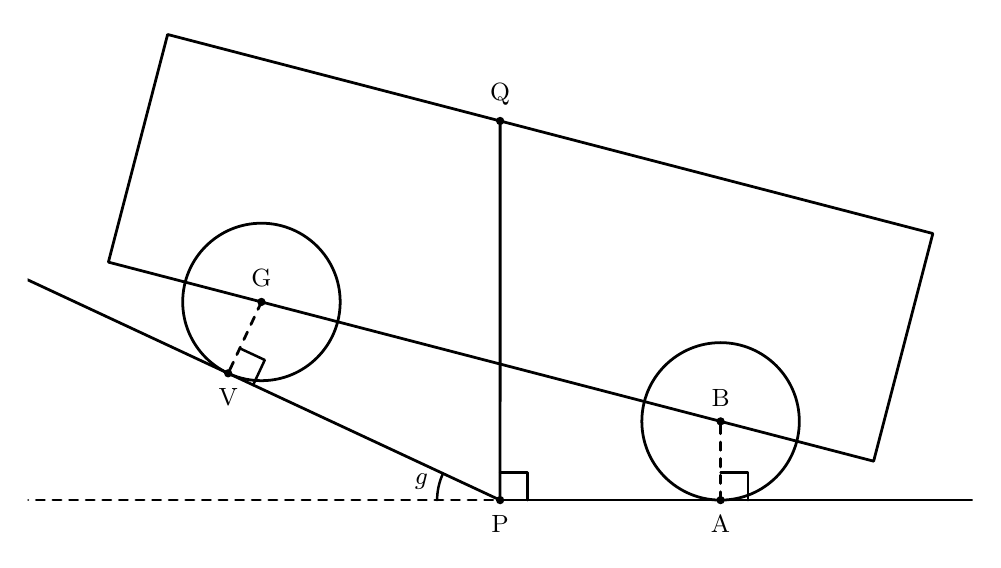
\begin{tikzpicture}[x=1cm,y=1cm,font=\small,line cap=round,line join=round]

\clip (-6,-.5) rectangle (6,6);
% \path[use as bounding box] (-8,-2) rectangle (10,5);



% x=1cm, y=1cm : giữ đúng tỉ lệ 1:1 giữa trục x và y (không méo hình)
% line cap / join bo tròn cho nét vẽ mềm hơn

% ===================== Parameters =====================
\pgfmathsetmacro{\alpha}{25}
% alpha: góc dốc (đơn vị: độ)
% dốc nghiêng lên về bên trái, hợp với mặt đường một góc g = alpha

\pgfmathsetmacro{\rW}{1}
% rW: bán kính bánh xe

\pgfmathsetmacro{\Lwb}{6}
% Lwb: wheelbase = khoảng cách giữa hai tâm bánh (|BG|)

\pgfmathsetmacro{\tFront}{2.8}
% tFront: hoành độ điểm A
% A là điểm tiếp xúc của bánh trước với mặt đường phẳng (y = 0)
% tăng tFront → xe tiến sang phải
% giảm tFront → xe lùi về trái (gần điểm P hơn)

\pgfmathsetmacro{\Hbody}{85}
% Hbody: chiều cao thùng xe
% đo theo phương vuông góc với trục bánh (GB), KHÔNG phải phương thẳng đứng

\pgfmathsetmacro{\ohRear}{2}
% ohRear: phần thùng xe thò ra phía sau bánh sau

\pgfmathsetmacro{\ohFront}{2}
% ohFront: phần thùng xe thò ra phía trước bánh trước

% ======================================================

% Các giá trị lượng giác của alpha (TikZ tính theo độ)
\pgfmathsetmacro{\cA}{cos(\alpha)}  % cos(alpha)
\pgfmathsetmacro{\sA}{sin(\alpha)}  % sin(alpha)
\pgfmathsetmacro{\mA}{tan(\alpha)}  % tan(alpha)

% ------------------------------------------------------
% P là điểm nối giữa mặt đường phẳng và con dốc
\coordinate (P) at (0,0);

% --- Mặt đường phẳng ---
\draw[dashed, line width=1.0pt] (-8,0) -- (P);
% đoạn đường nằm dưới dốc (bị che khuất) → nét đứt

\draw[line width=1.0pt] (P) -- (8,0);
% đoạn đường lộ ra dưới gầm cầu → nét liền

% --- Con dốc ---
% Phương trình: y = -tan(alpha) * x
% Dốc nghiêng lên về bên trái
\draw[line width=1.0pt] (-8,{ -\mA*(-8) }) -- (P);

% ------------------------------------------------------
% Bánh trước

\coordinate (A) at (\tFront,0);
% A: điểm tiếp xúc bánh trước với mặt đường

\coordinate (B) at (\tFront,\rW);
% B: tâm bánh trước, cách A một đoạn rW theo phương thẳng đứng

% ------------------------------------------------------
% Bánh sau (phần quan trọng nhất về hình học)

% Ý tưởng:
% - V là điểm tiếp xúc bánh sau với dốc
% - G là tâm bánh sau
% - |BG| = Lwb (wheelbase cố định)
%
% Tham số hóa:
% V = (-s cos(alpha), s sin(alpha))
% G = V + rW (sin(alpha), cos(alpha))

% Các hệ số của phương trình bậc hai theo s
\pgfmathsetmacro{\Bq}{2*( \tFront*\cA - \rW*\sA - \rW*\sA*(1-\cA) )}
\pgfmathsetmacro{\Cq}{(\tFront - \rW*\sA)^2 + (\rW*(1-\cA))^2 - (\Lwb)^2}

\pgfmathsetmacro{\Disc}{(\Bq)^2 - 4*(\Cq)}
% Disc: biệt thức Δ
% Nếu Disc < 0 → không tồn tại vị trí bánh sau (sqrt bị lỗi)

\pgfmathsetmacro{\sParam}{(-\Bq + sqrt(\Disc))/2}
% sParam: nghiệm dương, tương ứng vị trí bánh sau nằm về bên trái P

% Tọa độ điểm tiếp xúc và tâm bánh sau
\coordinate (V) at ({-\sParam*\cA},{\sParam*\sA});
\coordinate (G) at ({-\sParam*\cA + \rW*\sA},{\sParam*\sA + \rW*\cA});

% ------------------------------------------------------
% Vẽ bánh xe

\draw[line width=1.0pt] (G) circle (\rW);
\draw[line width=1.0pt] (B) circle (\rW);

\fill (A) circle (1.5pt);
\fill (B) circle (1.5pt);
\fill (V) circle (1.5pt);
\fill (G) circle (1.5pt);

\node[below=2pt] at (A) {A};
\node[above=2pt] at (B) {B};
\node[below=2pt] at (V) {V};
\node[above=2pt] at (G) {G};

\draw[dashed, line width=1.0pt] (A) -- (B);
% Dấu vuông góc tại P
\draw[line width=0.9pt]
  ($(A)+(0,0.35)$) -- ($(A)+(0.35,0.35)$) -- ($(A)+(0.35,0)$);

\draw[dashed, line width=1.0pt] (G) -- (V);
% Dấu vuông góc tại P
\draw[line width=0.9pt, rotate=-\alpha]
  ($(V)+(0,0.35)$) -- ($(V)+(0.35,0.35)$) -- ($(V)+(0.35,0)$);

% ------------------------------------------------------
% Vector trục bánh và pháp tuyến của nó

\path let \p1=($(B)-(G)$), \n1={veclen(\x1,\y1)} in
  coordinate (u)  at ($ (0,0) + (\x1/\n1,\y1/\n1) $)
  % u: vector đơn vị theo hướng trục bánh (từ G đến B)

  coordinate (nU) at ($ (0,0) + (-\y1/\n1,\x1/\n1) $);
  % nU: vector đơn vị vuông góc trục bánh

% ------------------------------------------------------
% Thùng xe (hình chữ nhật, dài hơn wheelbase)

% Quy đổi overhang sang tham số nội suy trên đoạn GB
\pgfmathsetmacro{\tRear}{-\ohRear/\Lwb}
% tRear < 0 → kéo lùi qua phía sau G

\pgfmathsetmacro{\tFront}{1+\ohFront/\Lwb}
% tFront > 1 → kéo vượt qua phía trước B

\coordinate (RB) at ($(G)!\tRear!(B)$);
% RB: góc đáy phía sau thùng xe

\coordinate (FB) at ($(G)!\tFront!(B)$);
% FB: góc đáy phía trước thùng xe

% Cạnh trên của thùng xe
\coordinate (RT) at ($(RB) + \Hbody*(nU)$);
\coordinate (FT) at ($(FB) + \Hbody*(nU)$);

% Vẽ hình chữ nhật thùng xe
\draw[line width=1.0pt] (RB) -- (FB) -- (FT) -- (RT) -- cycle;

% Đường mảnh song song đáy (tạo cảm giác hai nét)
% \draw[line width=0.9pt] ($(RB) + 0.10*(nU)$) -- ($(FB) + 0.10*(nU)$);

% ------------------------------------------------------
% PQ: đường thẳng đứng tại P, vuông góc mặt đường

\path[name path=topEdge] (RT) -- (FT);
% cạnh trên thùng xe

\path[name path=vertP] (P) -- ($(P)+(0,10)$);
% đường thẳng đứng qua P

\path[name intersections={of=topEdge and vertP, by=Q}];
% Q là giao điểm của PQ với cạnh trên thùng xe
% (nếu không cắt → sẽ báo lỗi intersections)

\fill (P) circle (1.5pt);
\fill (Q) circle (1.5pt);

\draw[line width=1.0pt] (P) -- (Q);

\node[above=2pt] at (Q) {Q};
\node[below=2pt] at (P) {P};

% Dấu vuông góc tại P
\draw[line width=0.9pt]
  ($(P)+(0,0.35)$) -- ($(P)+(0.35,0.35)$) -- ($(P)+(0.35,0)$);

% ------------------------------------------------------
% Góc g giữa dốc và mặt đường

\coordinate (Xroad) at ($(P)-(1,0)$);
% điểm xác định hướng mặt đường

\coordinate (Xslope) at ($(P)+(-1,{\mA})$);
% điểm xác định hướng dốc

\pic[draw, line width=0.9pt, angle radius=8mm]
  {angle=Xslope--P--Xroad};

\node at ($(P)+(-1,{\mA/2})$) {$g$};

\end{tikzpicture}
\end{document}
